%!TEX root = ../StrinJet.tex

\section{Simulate with PYTHIA 8 sQCD with CR1 and rope}%
\label{sec:Parameter}


\textbf{Parameters}

Beams:idA = 2212
\\Beams:idB = 2212
\\Main:numberOfEvents = 1001
\\Beams:eCM = 7000.
\\SoftQCD:all = on
\\
\\\textbf{CR}
\\MultiPartonInteractions:pT0Ref = 2.15
\\BeamRemnants:remnantMode = 1
\\BeamRemnants:saturation = 5
\\ColourReconnection:reconnect = on
\\ColourReconnection:mode = 1
\\ColourReconnection:allowDoubleJunRem = off
\\ColourReconnection:m0 = 0.3
\\ColourReconnection:allowJunctions = on
\\ColourReconnection:junctionCorrection = 1.2
\\ColourReconnection:timeDilationMode = 2
\\ColourReconnection:timeDilationPar = 0.18
\\
\\\textbf{Rope}
\\Ropewalk:RopeHadronization = on
\\Ropewalk:doShoving = on
\\Ropewalk:tInit = 1.5 %# Propagation time
\\Ropewalk:deltat = 0.05
\\Ropewalk:tShove = 0.1
\\Ropewalk:gAmplitude = 0. %# Set shoving strength to 0 explicitly
\\
\\Ropewalk:doFlavour = on
\\Ropewalk:r0 = 0.5
\\Ropewalk:m0 = 0.2
\\Ropewalk:beta = 0.1
\\
\\!// Enabling setting of vertex information.
\\PartonVertex:setVertex = on
\\PartonVertex:protonRadius = 0.7
\\PartonVertex:emissionWidth = 0.1


%\begin{figure}[ht]
%	\begin{center}
%		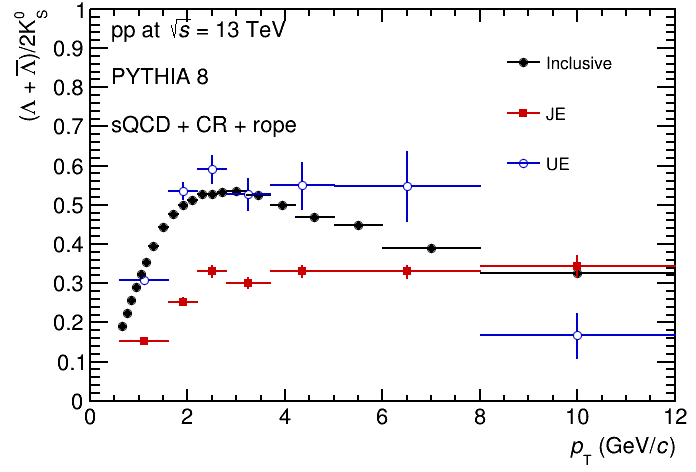
\includegraphics[width=.32\textwidth]{LKRatio_sQCD_CR_rope}
%		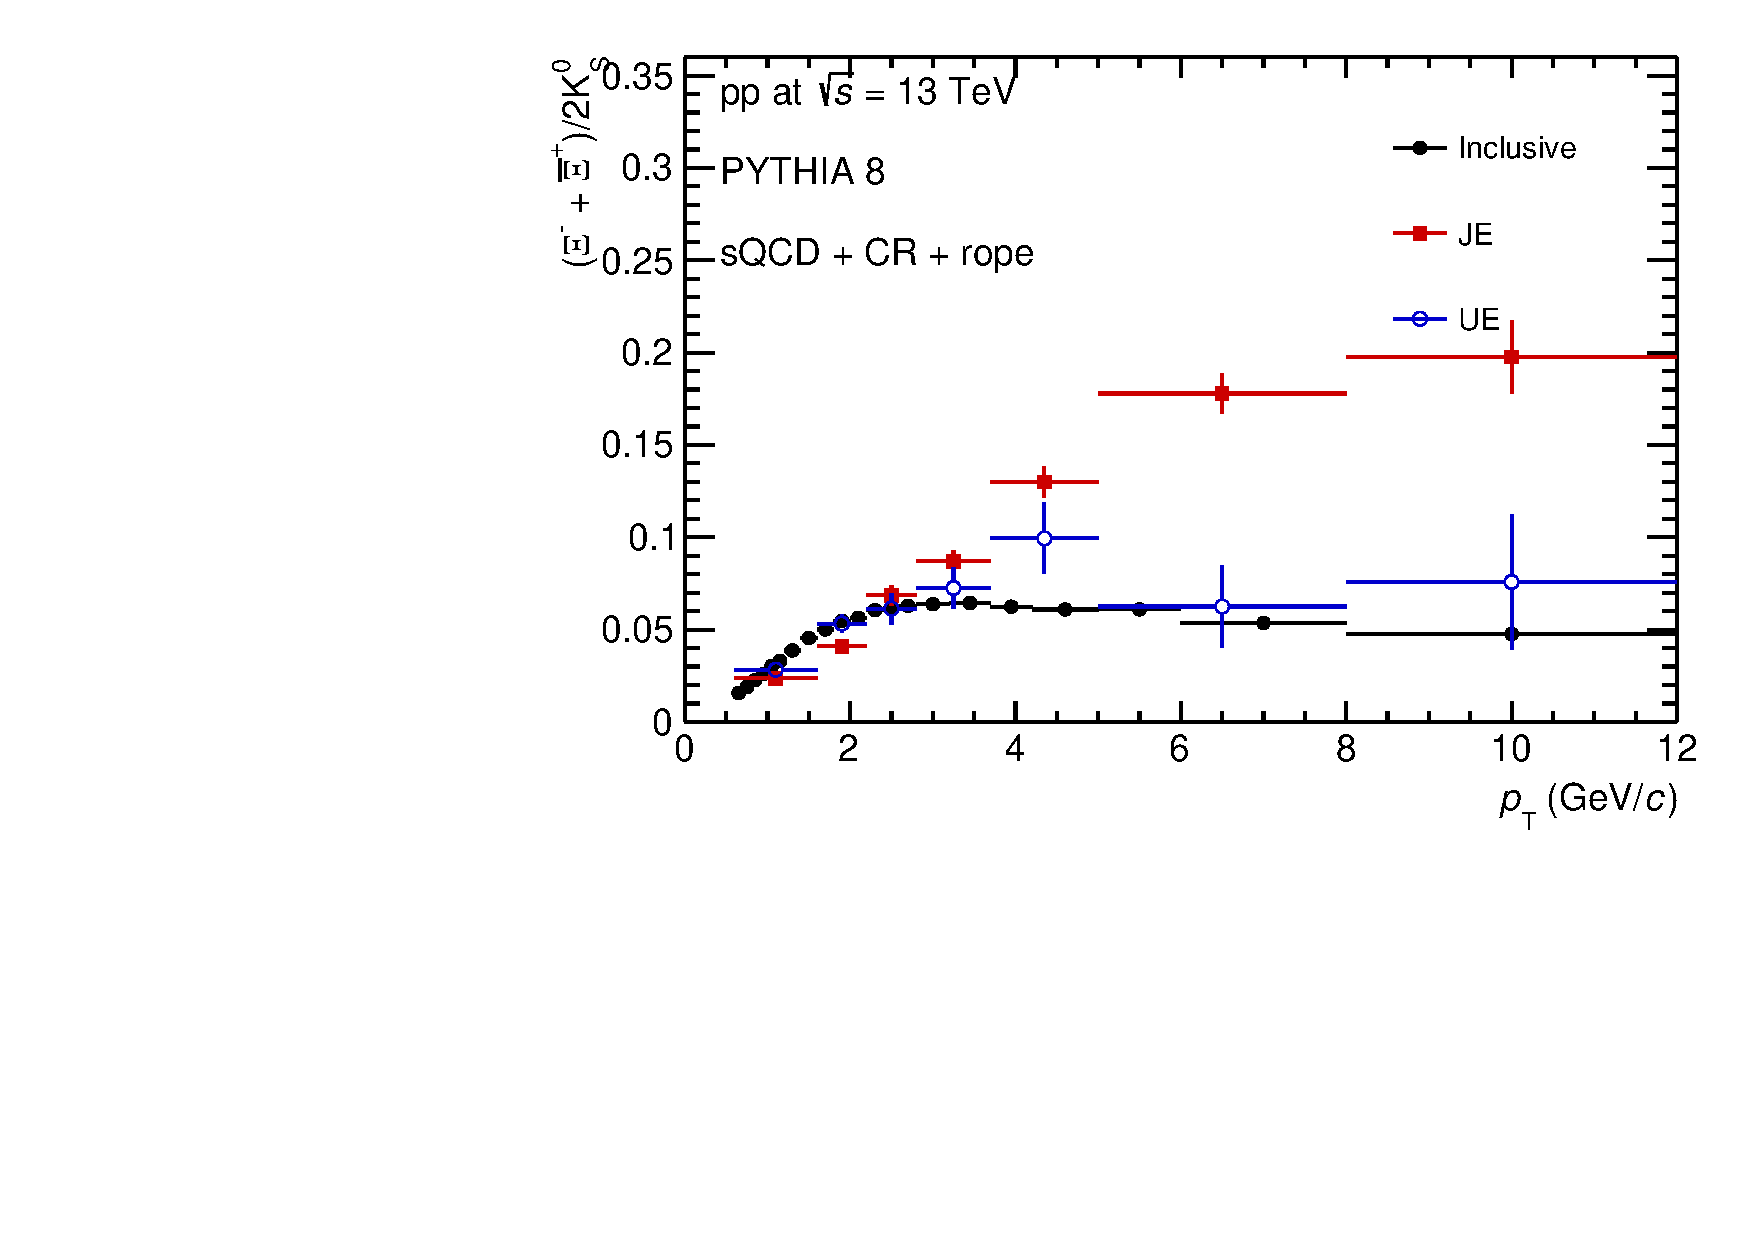
\includegraphics[width=.32\textwidth]{XKRatio_sQCD_CR_rope}
%		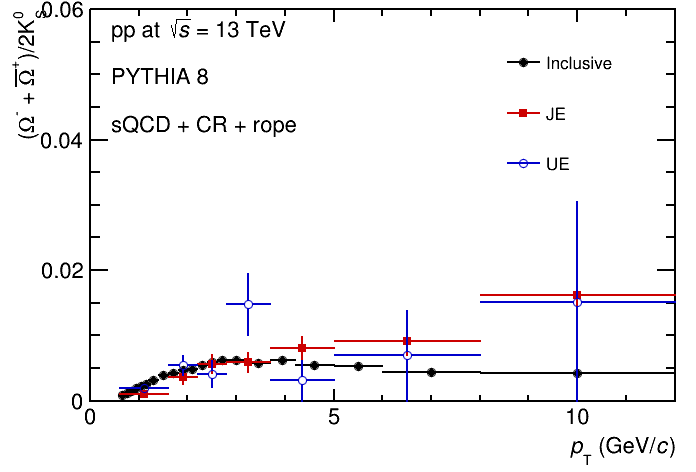
\includegraphics[width=.32\textwidth]{OKRatio_sQCD_CR_rope}
%		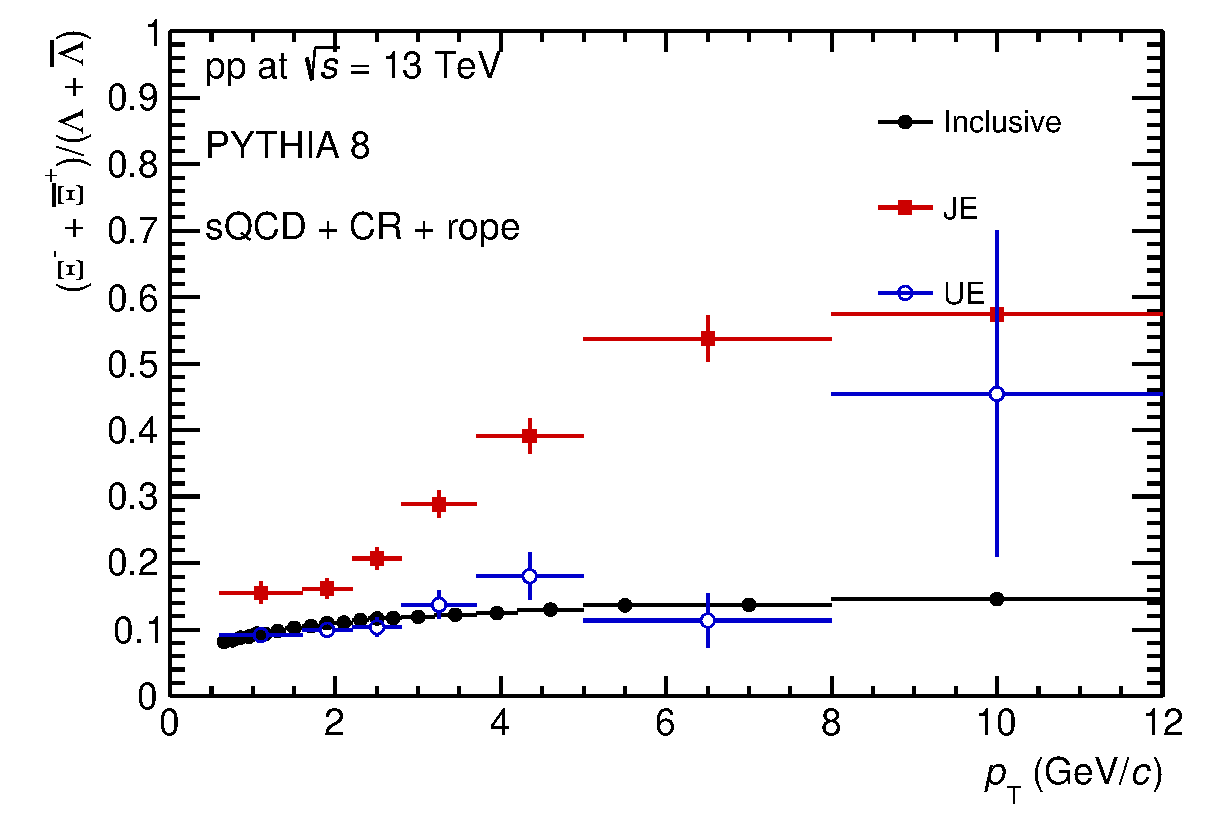
\includegraphics[width=.32\textwidth]{XLRatio_sQCD_CR_rope}
%%		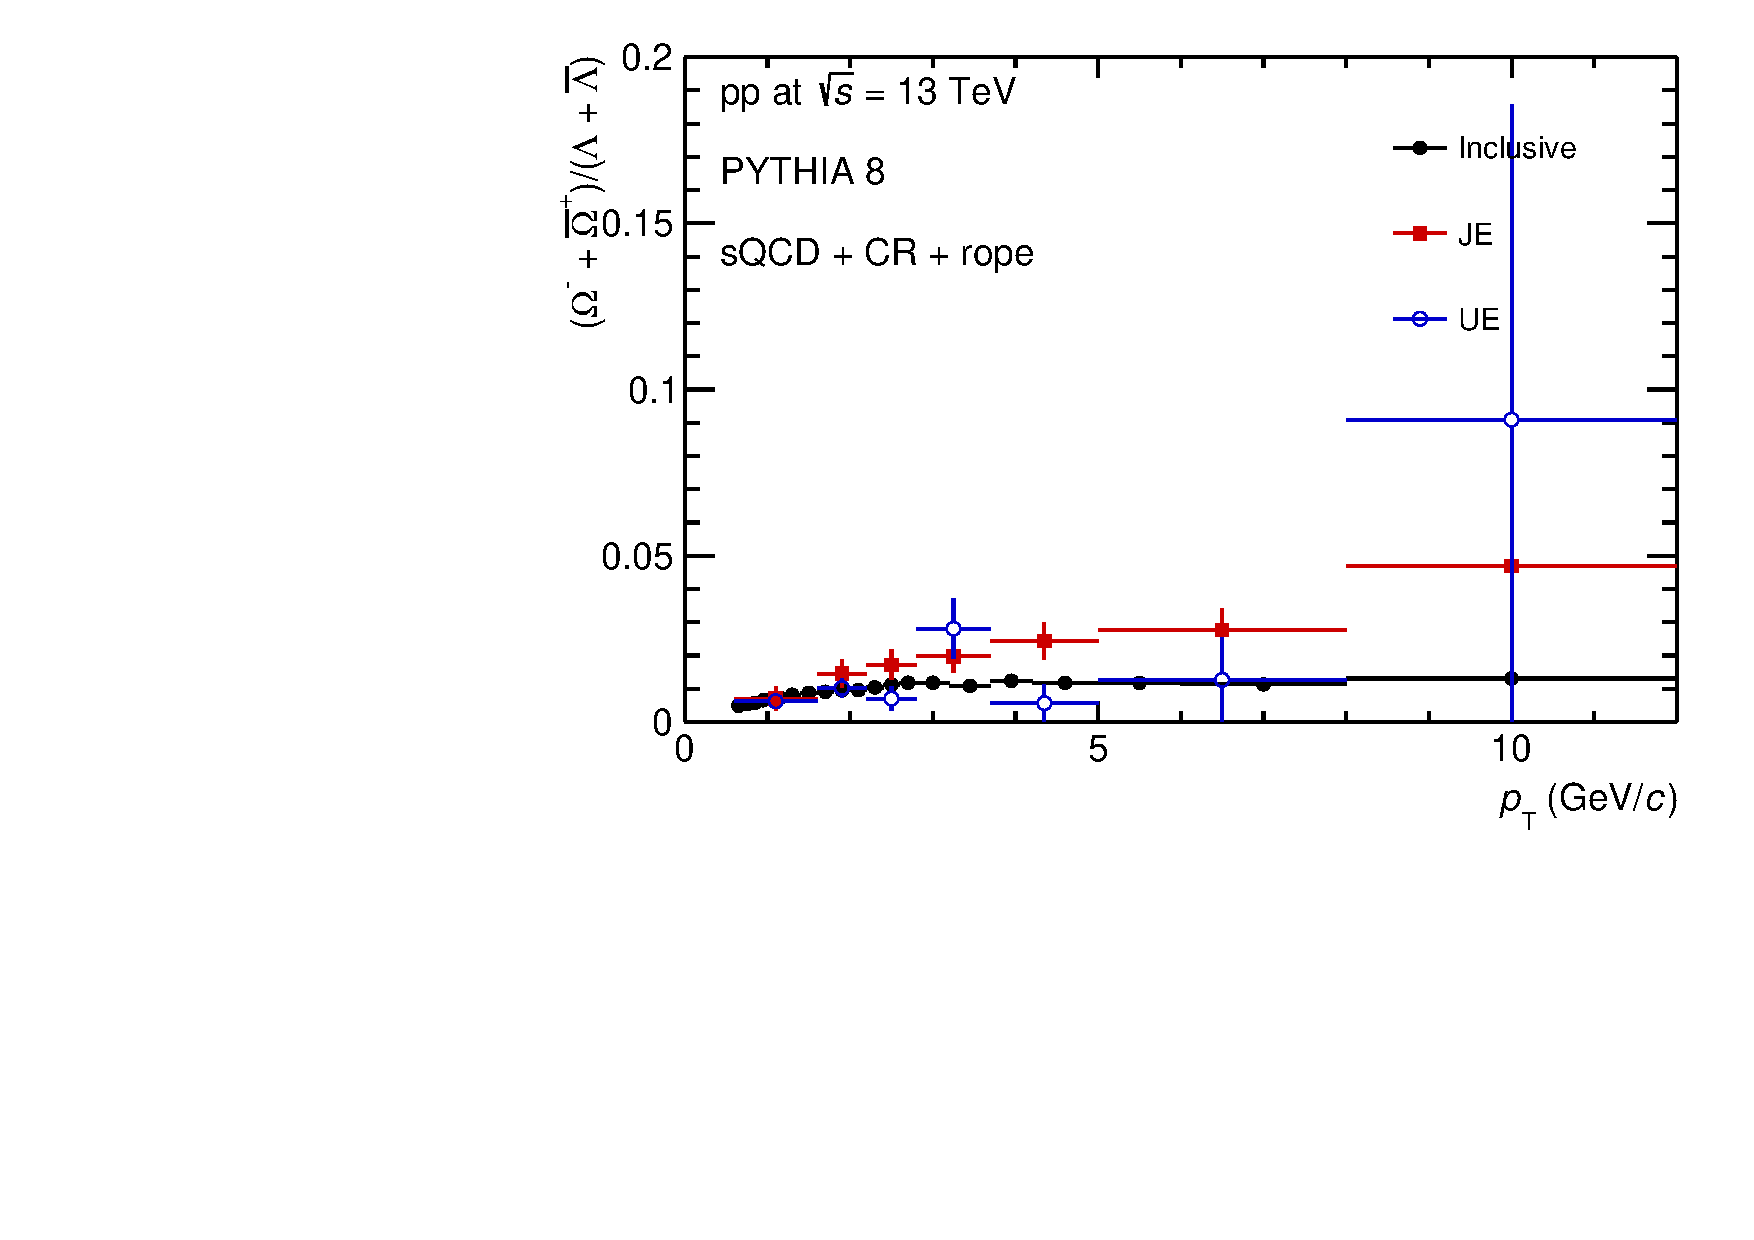
\includegraphics[width=.32\textwidth]{OLRatio_sQCD_CR_rope}
%		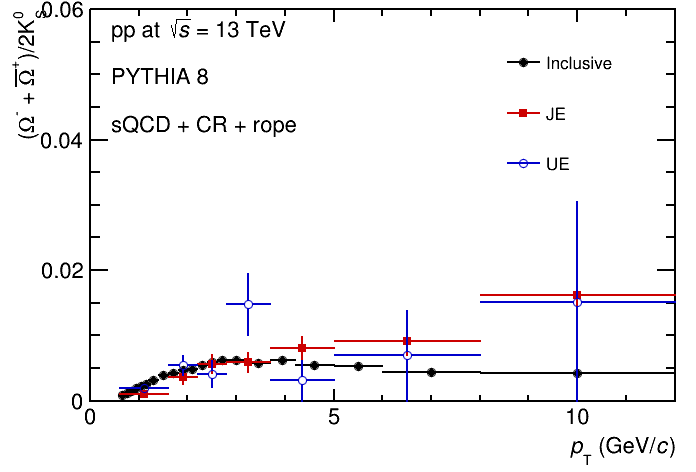
\includegraphics[width=.32\textwidth]{OKRatio_sQCD_CR_rope}
%	\end{center}
%	\caption{Baryon-to-meson(top) and baryon-to-baryon ratio with PYTHIA sQCD + CR1 + rope.}
%	\label{fig:ParticleRatiowithCRandRope}
%\end{figure}